\documentclass{standalone}
\usepackage{tikz}
\usepackage{hsbcommon}
\begin{document}
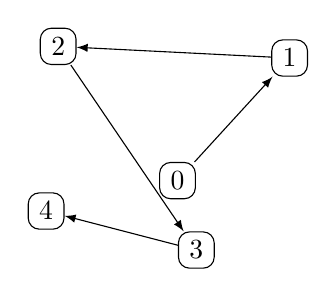
\begin{tikzpicture}
    \tikzset{
        every node/.style={
            minimum width=3ex,
            minimum height=3ex,
            draw, rounded corners,
            fill=white
            }
    }
     \def\myx{}
     \def\myy{}
     \def\mya{}
     \def\myb{}
        \pgfmathsetseed{4}
    \node (N0) at (2.5,2.5) {0};
    \foreach [count=\i] \ii in {0,...,3}
    {
        \pgfmathsetmacro\myx{rnd*(5)}
        \pgfmathsetmacro\myy{rnd*(5)}
        \node (N\i) at (\myx,\myy) {\i};
        \draw[->,>=latex] (N\ii) -- (N\i) ;
    }
\end{tikzpicture}
\end{document}